\documentclass[../main.tex]{subfiles}
\begin{document}
%=========================================================
% TĐ_PBT_IQA_HK1_Tuan18_OnTapCuoiHK1
% Phiếu bài tập Toán tư duy cấp độ A - Chủ đề ÔN TẬP CUỐI HỌC KÌ 1 (Buổi 1, Buổi 2)
% Bài tập bổ sung, mức độ cơ bản - trung bình, mọi hình vẽ bằng TikZ (không dùng ảnh ngoài)
% Soạn theo mẫu (\hktuan, bt, listEX) như các phiếu Tuần 15, 16
%=========================================================

%---------- Lệnh dùng riêng cho phiếu ----------
\providecommand{\TTcham}{}\renewcommand{\TTcham}[1][3cm]{\makebox[#1]{\dotfill}}
\providecommand{\TTthongtin}{%
  \noindent\begin{tabular}{|p{7.6cm}|p{4cm}|p{4cm}|}
    \hline
    \textbf{Họ và Tên HS:}\dotfill & \textbf{Lớp:}\dotfill & \textbf{Ngày:}\dotfill \\
    \hline
  \end{tabular}\par\medskip}
\makeatletter
\providecommand{\TTdatlaibai}{\@ifundefined{c@bt}{}{\setcounter{bt}{0}}}
\makeatother
% Phương án trắc nghiệm A, B, C thẳng hàng giữa các câu
\providecommand{\OTchon}{}\renewcommand{\OTchon}[3]{\par\noindent\hspace*{1cm}%
  \makebox[0.3\linewidth][l]{\textbf{A.}~#1}%
  \makebox[0.3\linewidth][l]{\textbf{B.}~#2}%
  \makebox[0.3\linewidth][l]{\textbf{C.}~#3}\par}
% Ô vuông nhỏ để ghi Đ/S hoặc điền kết quả
\providecommand{\OTovuong}{}\renewcommand{\OTovuong}[1][0.42cm]{\fbox{\rule{0pt}{#1}\rule{#1}{0pt}}}
% Khung viết phép tính cho bài toán có lời văn
\providecommand{\OTkhungpt}{}\renewcommand{\OTkhungpt}{\par\medskip\noindent
  \textbf{Phép tính:}\ \framebox[4.6cm][l]{\rule{0pt}{0.85cm}}\hspace{0.6cm}\textbf{Đáp số:}\ \framebox[3.2cm][l]{\rule{0pt}{0.85cm}}\par\smallskip}

%---------- Màu và kiểu chung (dùng được cả khi in trắng đen) ----------
\definecolor{OTxanh}{RGB}{120,190,235}\definecolor{OTxanhdam}{RGB}{25,95,170}
\definecolor{OTcam}{RGB}{250,170,70}\definecolor{OTcamdam}{RGB}{200,90,20}
\definecolor{OTvang}{RGB}{255,225,130}\definecolor{OTvangnhat}{RGB}{255,246,205}
\definecolor{OThong}{RGB}{245,150,175}\definecolor{OTla}{RGB}{125,195,120}
\definecolor{OTtim}{RGB}{185,160,225}\definecolor{OTnau}{RGB}{120,75,35}
\tikzset{
  OTo/.style={draw=black!80,thick,rounded corners=3pt,minimum width=0.95cm,minimum height=0.8cm,inner sep=0pt,font=\sffamily\bfseries\large},
  OTotron/.style={draw=black!80,thick,circle,minimum size=1.0cm,inner sep=0pt,font=\sffamily\bfseries\large},
  OTgach/.style={draw=OTcamdam,thick,fill=OTcam!35,minimum width=1.5cm,minimum height=0.8cm,inner sep=0pt,font=\sffamily\bfseries\large},
  OTthe/.style={draw=OTxanhdam,thick,rounded corners=5pt,fill=OTxanh!20,minimum width=1.3cm,minimum height=0.95cm,inner sep=0pt,font=\sffamily\bfseries\Large},
}

% Dãy ô số: \OTday{a,b,,d,...} (để trống = ô cần điền)
\providecommand{\OTday}{}\renewcommand{\OTday}[1]{%
  \begin{tikzpicture}\foreach \x [count=\k] in {#1}{\node[OTo,minimum width=1.15cm,minimum height=0.9cm] at (1.25*\k,0) {\x};}\end{tikzpicture}}

% Bảng số liền trước / ở giữa / liền sau: \OTlt{tiêu đề}{kiểu 1,2,3}{a/b,c/d,...}
\providecommand{\OTlt}{}\renewcommand{\OTlt}[3]{%
  \begin{tikzpicture}[font=\sffamily\bfseries\large]
    \draw[thick,rounded corners=6pt,fill=black!4] (0,0.55) rectangle (4.3,-6.1);
    \node[draw,thick,rounded corners=4pt,fill=OTxanh!25,minimum width=3.7cm,minimum height=0.8cm,font=\sffamily\bfseries] at (2.15,0.0) {#1};
    \foreach \a/\b [count=\k] in {#3}{%
      \ifnum#2=1 \node[OTo,fill=white] at (1.0,-1.1*\k) {}; \node at (2.4,-1.1*\k) {\a};\fi
      \ifnum#2=2 \node at (0.7,-1.1*\k) {\a}; \node[OTo,fill=white] at (2.15,-1.1*\k) {}; \node at (3.6,-1.1*\k) {\b};\fi
      \ifnum#2=3 \node at (1.2,-1.1*\k) {\a}; \node[OTo,fill=white] at (2.9,-1.1*\k) {};\fi}
  \end{tikzpicture}}

% Hoa ghi số (để tô màu): \OThoa{số}{màu cánh}
\providecommand{\OThoa}{}\renewcommand{\OThoa}[2]{%
  \begin{tikzpicture}
    \foreach \a in {90,162,234,306,18}{%
      \begin{scope}[rotate=\a]\draw[fill=#2,draw=black!70,thick] (0.52,0) ellipse (0.4 and 0.3);\end{scope}}
    \draw[fill=white,draw=black!70,thick] (0,0) circle (0.42);
    \node[font=\sffamily\bfseries\large] at (0,0) {#1};
  \end{tikzpicture}}

% Trái tim ghi số: \OTtim{số}
\providecommand{\OTtim}{}\renewcommand{\OTtim}[1]{%
  \begin{tikzpicture}
    \draw[thick,fill=OThong!35,draw=black!75,line join=round]
      (0,-0.62) .. controls (-0.2,-0.45) and (-0.95,-0.05) .. (-0.95,0.32)
      .. controls (-0.95,0.72) and (-0.4,0.88) .. (0,0.5)
      .. controls (0.4,0.88) and (0.95,0.72) .. (0.95,0.32)
      .. controls (0.95,-0.05) and (0.2,-0.45) .. (0,-0.62) -- cycle;
    \fill[white,opacity=0.6] (-0.55,0.45) ellipse (0.14 and 0.08);
    \node[font=\sffamily\bfseries\large] at (0,0.12) {#1};
  \end{tikzpicture}}

% Quả bí ngô có phép tính: \OTbingo{phép tính}
\providecommand{\OTbingo}{}\renewcommand{\OTbingo}[1]{%
  \begin{tikzpicture}
    \foreach \dx in {-0.5,0.5,-0.25,0.25}{\draw[fill=OTcam!75!yellow,draw=OTcamdam,thick] (\dx,0) ellipse (0.5 and 0.62);}
    \draw[fill=OTcam!75!yellow,draw=OTcamdam,thick] (0,0) ellipse (0.45 and 0.62);
    \draw[OTcamdam,thin] (-0.25,0.52) .. controls (-0.3,0) .. (-0.25,-0.52) (0.25,0.52) .. controls (0.3,0) .. (0.25,-0.52);
    \draw[draw=OTnau,fill=OTnau!70!OTla,thick,rounded corners=1.5pt] (-0.07,0.58)--(-0.05,0.9)--(0.14,0.95)--(0.13,0.58)--cycle;
    \draw[draw=OTla!50!black,fill=OTla,thick] (0.14,0.78) .. controls (0.5,1.05) and (0.7,0.8) .. (0.45,0.68) .. controls (0.35,0.72) .. (0.14,0.78);
    \node[fill=white,rounded corners=2pt,inner sep=2pt,font=\sffamily\bfseries\large] at (0,-0.03) {#1};
  \end{tikzpicture}}

% Cây tách số: \OTtach{số}{trái}{phải}
\providecommand{\OTtach}{}\renewcommand{\OTtach}[3]{%
  \begin{tikzpicture}
    \node[OTotron,fill=OTvang] (t) at (0,0) {#1};
    \node[OTotron,fill=white] (l) at (-0.95,-1.45) {#2};
    \node[OTotron,fill=white] (r) at (0.95,-1.45) {#3};
    \draw[thick] (t)--(l) (t)--(r);
  \end{tikzpicture}}

% Đồng hồ: \OTdh[1 = vẽ kim, 0 = mặt trống]{giờ}{phút}
\providecommand{\OTdh}{}\renewcommand{\OTdh}[3][1]{%
  \begin{tikzpicture}
    \draw[draw=OTcamdam,line width=1.8pt,fill=OTvangnhat] (0,0) circle (1.08);
    \draw[draw=OTcam,line width=0.6pt] (0,0) circle (0.98);
    \foreach \k in {1,...,60}{\draw[black!55,line width=0.3pt] ({90-6*\k}:0.98)--({90-6*\k}:0.93);}
    \foreach \k in {1,...,12}{\draw[black!75,line width=0.8pt] ({90-30*\k}:0.98)--({90-30*\k}:0.88);}
    \foreach \k in {1,...,12}{\node[font=\sffamily\bfseries\fontsize{7}{8}\selectfont] at ({90-30*\k}:0.77) {\k};}
    \ifnum#1=1
      \pgfmathsetmacro{\OTag}{90-30*(#2+#3/60)}\pgfmathsetmacro{\OTam}{90-6*#3}
      \draw[line width=2.8pt,line cap=round,black!85] (0,0)--(\OTag:0.36);
      \draw[line width=1.6pt,line cap=round,OTxanhdam] (0,0)--(\OTam:0.57);
    \fi
    \fill[black!85] (0,0) circle (0.065);
  \end{tikzpicture}}

% Chuỗi phép tính: \OTchuoi{số đầu}{phép 1}{phép 2}
\providecommand{\OTchuoi}{}\renewcommand{\OTchuoi}[3]{%
  \begin{tikzpicture}[font=\sffamily\bfseries\large]
    \node[OTotron,fill=OTvang] (a) at (0,0) {#1};
    \node[OTo,minimum width=1.1cm,minimum height=0.95cm] (b) at (4.2,0) {};
    \node[OTo,minimum width=1.1cm,minimum height=0.95cm] (c) at (8.4,0) {};
    \draw[-latex,thick] (a.east)--node[above=2pt,fill=white,inner sep=1pt]{#2} (b.west);
    \draw[-latex,thick] (b.east)--node[above=2pt,fill=white,inner sep=1pt]{#3} (c.west);
  \end{tikzpicture}}

% Cột phép tính trong khung bo tròn: \OTcotpt{a,b,c,d,e}
\providecommand{\OTcotpt}{}\renewcommand{\OTcotpt}[1]{%
  \begin{tikzpicture}[font=\sffamily\large]
    \draw[thick,rounded corners=10pt,fill=black!3] (0,0.3) rectangle (5.3,-4.7);
    \foreach \pt [count=\k] in {#1}{\node[anchor=west] at (0.3,-0.9*\k+0.45) {$\pt =$\ \rule{1.4cm}{0.5pt}};}
  \end{tikzpicture}}

% Hình khối để đếm: \OThinh{loại}  (T tam giác, V vuông, N chữ nhật, C tròn) vẽ tại gốc tọa độ
\providecommand{\OThinh}{}\renewcommand{\OThinh}[1]{\csname OThinh#1\endcsname}
\def\OThinhT{\draw[thick,fill=OTcam!45,draw=OTcamdam,line join=round] (-0.5,-0.4)--(0.5,-0.4)--(0,0.45)--cycle;}
\def\OThinhV{\draw[thick,fill=OTxanh!45,draw=OTxanhdam,line join=round] (-0.42,-0.42) rectangle (0.42,0.42);}
\def\OThinhN{\draw[thick,fill=OTla!50,draw=OTla!40!black,line join=round] (-0.6,-0.3) rectangle (0.6,0.3);}
\def\OThinhC{\draw[thick,fill=OThong!50,draw=OThong!40!black] (0,0) circle (0.45);}


% Tiêu đề từng dạng bài
\providecommand{\OTdang}{}\renewcommand{\OTdang}[1]{\par\vspace{8pt}\noindent\colorbox{mauchinh!12}{\color{mauchinh}\bfseries\ #1\ }\par\nopagebreak\vspace{2pt}}

% Tia số: \OTtia{số lớn nhất}{bước ghi nhãn}{độ dài 1 đơn vị (cm)}; vẽ trong tikzpicture
\providecommand{\OTtia}{}\renewcommand{\OTtia}[3]{%
  \draw[thick,-latex] (-0.35,0)--({#1*#3+0.55},0);
  \foreach \k in {0,#2,...,#1}{\draw[thick] ({\k*#3},-0.12)--({\k*#3},0.12);
    \node[font=\sffamily\bfseries\small] at ({\k*#3},-0.45) {\k};}}
% Cung nhảy trên tia số: \OTcung{từ}{đến}{độ dài đơn vị}{nhãn}{hướng: bend left/right}
\providecommand{\OTcung}{}\renewcommand{\OTcung}[5]{%
  \draw[-latex,very thick,OTxanhdam] ({#1*#3},0.14) to[#5=65] node[above=1pt,font=\sffamily\bfseries\small,fill=white,inner sep=1pt]{#4} ({#2*#3},0.14);}

% Ngôi nhà số: \OTnhaso{số mái}{cửa sổ trái}{cửa sổ phải}
\providecommand{\OTnhaso}{}\renewcommand{\OTnhaso}[3]{%
  \begin{tikzpicture}[font=\sffamily\bfseries\large]
    \draw[thick,fill=OTcam!30,draw=OTcamdam,line join=round] (-1.15,1.4)--(0,2.5)--(1.15,1.4)--cycle;
    \draw[thick,fill=OTvangnhat,draw=black!75] (-0.95,0) rectangle (0.95,1.4);
    \node at (0,1.78) {#1};
    \node[draw=black!80,thick,fill=white,minimum size=0.6cm,inner sep=0pt] at (-0.45,0.7) {#2};
    \node[draw=black!80,thick,fill=white,minimum size=0.6cm,inner sep=0pt] at (0.45,0.7) {#3};
  \end{tikzpicture}}

% Quả táo, quả bóng bay (vẽ tại gốc tọa độ)
\providecommand{\OTtao}{}\renewcommand{\OTtao}{%
  \fill[red!80!black!85,draw=red!50!black,thin] (-0.1,0) circle (0.2) (0.1,0) circle (0.2);
  \draw[draw=OTnau,thick] (0,0.15)--(0.02,0.3);
  \fill[OTla!85!black,rotate around={25:(0.1,0.28)}] (0.11,0.28) ellipse (0.1 and 0.045);
  \fill[white,opacity=0.55] (-0.15,0.05) ellipse (0.04 and 0.07);}
\providecommand{\OTbongbay}{}\renewcommand{\OTbongbay}[1][OTxanh]{%
  \fill[#1,draw=black!60,thin] (0,0.1) ellipse (0.2 and 0.26);
  \fill[black!60] (0,-0.17)--(-0.04,-0.23)--(0.04,-0.23)--cycle;
  \draw[black!50,thin] (0,-0.23) .. controls (-0.1,-0.35) and (0.1,-0.4) .. (0,-0.5);
  \fill[white,opacity=0.6] (-0.08,0.18) ellipse (0.035 and 0.07);}
% Gạch chéo (bớt đi) lên một biểu tượng
\providecommand{\OTgach}{}
\providecommand{\OTcheo}{}\renewcommand{\OTcheo}{\draw[very thick,black] (-0.24,-0.24)--(0.24,0.24) (-0.24,0.24)--(0.24,-0.24);}
% Hàng biểu tượng: \OThang{\biểu tượng}{số lượng}{số bị gạch}
\providecommand{\OThang}{}\renewcommand{\OThang}[3]{%
  \foreach \k in {1,...,#2}{\begin{scope}[shift={(0.62*\k,0)}]#1\ifnum\k>\numexpr#2-#3\relax\OTcheo\fi\end{scope}}}

% Bảng cộng: \OTbangcong{các số cột}{các số hàng}
\providecommand{\OTbangcong}{}\renewcommand{\OTbangcong}[2]{%
  \begin{tikzpicture}[font=\sffamily\bfseries\large]
    \node[draw=black!80,thick,fill=OTvang,minimum width=1.3cm,minimum height=0.9cm] (g) at (0,0) {$+$};
    \foreach \c [count=\i] in {#1}{\node[draw=black!80,thick,fill=OTxanh!30,minimum width=1.3cm,minimum height=0.9cm] at (1.3*\i,0) {\c};}
    \foreach \r [count=\j] in {#2}{\node[draw=black!80,thick,fill=OTxanh!30,minimum width=1.3cm,minimum height=0.9cm] at (0,-0.9*\j) {\r};
      \foreach \i in {1,...,5}{\node[draw=black!80,thick,fill=white,minimum width=1.3cm,minimum height=0.9cm] at (1.3*\i,-0.9*\j) {};}}
  \end{tikzpicture}}

% Thẻ phép tính để tô màu: \OTthepc{phép tính}
\providecommand{\OTthepc}{}\renewcommand{\OTthepc}[1]{\node[draw=black!70,very thick,rounded corners=6pt,fill=white,minimum width=2.4cm,minimum height=1.15cm,font=\sffamily\bfseries\large] {#1};}

% Một dòng phép tính điền ô: \OTpt{...} (chữ số cùng font)
\providecommand{\OTb}{}\renewcommand{\OTb}{\OTovuong[0.55cm]}

%%%%%%%%%%%%%%%%%%%%%%%%%%%%%
% BUỔI 1
%%%%%%%%%%%%%%%%%%%%%%%
\hktuan{1}{18}
\par\medskip
{\centering
        {\color{mauchinh!120}\bfseries\Large PHIẾU BÀI TẬP TOÁN TƯ DUY CẤP ĐỘ A}\\[3pt]
        {\color{mauchinh!120}\bfseries\Large CHỦ ĐỀ: ÔN TẬP CUỐI HỌC KÌ 1\\[2pt] PHẠM VI 20 (BUỔI 1)}\par}
\vspace{6pt}
\TTthongtin

\OTdang{DẠNG 1. CẤU TẠO SỐ VÀ TÁCH SỐ}
\begin{bt}
    Tách số rồi điền số thích hợp vào chỗ trống.
    \par\nopagebreak\vspace{4pt}\nopagebreak
    {\setlength{\tabcolsep}{2pt}\noindent\begin{tabular}{*{4}{>{\centering\arraybackslash}p{0.245\linewidth}}}
        \OTtach{11}{10}{} & \OTtach{14}{}{4} & \OTtach{19}{}{} & \OTtach{15}{}{} \\[8pt]
        \OTtach{12}{}{} & \OTtach{17}{7}{} & \OTtach{13}{}{3} & \OTtach{18}{}{} \\
    \end{tabular}\par}
\end{bt}
\begin{bt}
    Nối hai trái tim với nhau để có tổng bằng $10$.
    \par\nopagebreak\vspace{4pt}\nopagebreak{\centering
    \begin{tikzpicture}[font=\sffamily]
        \foreach \so/\y in {2/0,7/-1.55,9/-3.1,4/-4.65,5/-6.2}{\node at (0,\y) {\OTtim{\so}};\fill (1.25,\y) circle (2.5pt);}
        \foreach \so/\y in {6/0,5/-1.55,3/-3.1,8/-4.65,1/-6.2}{\node at (8,\y) {\OTtim{\so}};\fill (6.75,\y) circle (2.5pt);}
    \end{tikzpicture}\par}
\end{bt}
\OTdang{DẠNG 2. CỘNG, TRỪ TRONG PHẠM VI 20}
\begin{bt}
    Viết phép tính theo các bước nhảy trên tia số rồi tính.
    \par\nopagebreak\vspace{6pt}\nopagebreak{\centering
    
\begin{tikzpicture}[font=\sffamily\bfseries]
        \OTtia{20}{1}{0.62}
        \OTcung{8}{10}{0.62}{+2}{bend left}\OTcung{10}{13}{0.62}{+3}{bend left}
        \node[anchor=west,font=\sffamily\bfseries\large] at (-0.3,-1.25) {8 + 5 = \rule{1.2cm}{0.5pt}};
    \end{tikzpicture}\\[10pt]
    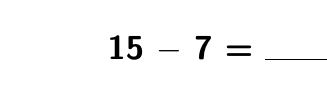
\begin{tikzpicture}[font=\sffamily\bfseries]
        \OTtia{20}{1}{0.62}
        \OTcung{15}{10}{0.62}{$-5$}{bend right}\OTcung{10}{8}{0.62}{$-2$}{bend right}
        \node[anchor=west,font=\sffamily\bfseries\large] at (-0.3,-1.25) {15 $-$ 7 = \rule{1.2cm}{0.5pt}};
    \end{tikzpicture}\\[10pt]
    \begin{tikzpicture}[font=\sffamily\bfseries]
        \OTtia{20}{1}{0.62}
        \node[anchor=west,font=\sffamily\bfseries\large] at (-0.3,-1.25) {Tự nhảy: 9 + 6 (nhảy từ 9 lên 10 rồi nhảy tiếp) = \rule{1.2cm}{0.5pt}};
    \end{tikzpicture}\par}
\end{bt}
\begin{bt}
    Cộng qua 10: điền số thích hợp vào ô trống.
    \begin{listEX}
        \item $8+5=8+\OTovuong+3=10+\OTovuong=\OTovuong$
        \item $9+6=9+\OTovuong+5=10+\OTovuong=\OTovuong$
        \item $7+8=7+\OTovuong+5=10+\OTovuong=\OTovuong$
        \item $6+9=\OTovuong+9=\OTovuong+\OTovuong=\OTovuong$
    \end{listEX}
\end{bt}
\begin{bt}
    Trừ qua 10: điền số thích hợp vào ô trống.
    \begin{listEX}
        \item $14-6=14-4-\OTovuong=10-\OTovuong=\OTovuong$
        \item $13-5=13-3-\OTovuong=10-\OTovuong=\OTovuong$
        \item $16-9=16-6-\OTovuong=10-\OTovuong=\OTovuong$
        \item $12-8=12-\OTovuong-\OTovuong=\OTovuong$
    \end{listEX}
\end{bt}
\begin{bt}
    Điền kết quả vào bảng cộng.
    \par\nopagebreak\vspace{4pt}\nopagebreak{\centering
        \OTbangcong{3,4,5,6,7}{5,6,7,8,9}\par}
\end{bt}
\begin{bt}
    Nối phép tính với kết quả đúng.
    \par\nopagebreak\vspace{4pt}\nopagebreak{\centering
    \begin{tikzpicture}[font=\sffamily\bfseries\large]
        \foreach \e/\y in {9+5/0,16-7/-1.3,8+8/-2.6,12-4/-3.9,7+6/-5.2}{
            \node[draw=black!80,thick,rounded corners=5pt,fill=OTvangnhat,minimum width=2.8cm,minimum height=0.85cm] at (0,\y) {\e};
            \fill (1.7,\y) circle (2.5pt);}
        \foreach \so/\y in {16/0,13/-1.3,9/-2.6,14/-3.9,8/-5.2}{
            \fill (5.3,\y) circle (2.5pt);
            \node[OTotron,fill=OTxanh!25,draw=OTxanhdam] at (6.4,\y) {\so};}
    \end{tikzpicture}\par}
\end{bt}
\begin{bt}
    Thực hiện phép tính.
    \par\nopagebreak\vspace{4pt}\nopagebreak{\centering
        \OTcotpt{6+7,8+9,5+6,9+9,4+8}\hfill
        \OTcotpt{9+4,15-6,12+5,18-8,7+8}\hfill
        \OTcotpt{16-9,6+9,14-5,5+13,20-12}\par}
\end{bt}
\begin{bt}
    Tính kết quả phép tính ghi trên mỗi quả bí ngô rồi điền vào ô trống.
    \par\nopagebreak\vspace{4pt}\nopagebreak{\centering
    \begin{tikzpicture}[font=\sffamily\bfseries\large]
        \foreach \e [count=\k] in {3+7,4+6,8+7,8+5,11+5,12+5}{
            \pgfmathtruncatemacro{\cot}{mod(\k-1,3)}\pgfmathtruncatemacro{\hang}{div(\k-1,3)}
            \begin{scope}[shift={(5.4*\cot,-2.1*\hang)}]
                \node at (0,0) {\OTbingo{\e}};
                \node[OTo,minimum width=1.5cm,minimum height=0.9cm] at (2.7,0) {};
            \end{scope}}
    \end{tikzpicture}\par}
\end{bt}
\OTdang{DẠNG 3. TÌM SỐ CÒN THIẾU, SO SÁNH, ĐIỀN DẤU}
\begin{bt}
    Tìm số còn thiếu (điền vào ô trống).
    \par\nopagebreak\vspace{6pt}\nopagebreak{\centering
    \renewcommand{\arraystretch}{2.0}
    \begin{tabular}{*{3}{>{\centering\arraybackslash}p{0.3\linewidth}}}
        $\OTovuong[0.7cm]+7=15$ & $13-\OTovuong[0.7cm]=6$ & $\OTovuong[0.7cm]-5=9$ \\
        $8+\OTovuong[0.7cm]=17$ & $16-\OTovuong[0.7cm]=9$ & $\OTovuong[0.7cm]+9=18$ \\
        $6+\OTovuong[0.7cm]=14$ & $\OTovuong[0.7cm]-8=7$ & $19-\OTovuong[0.7cm]=11$ \\
    \end{tabular}\par}
\end{bt}
\begin{bt}
    Điền dấu $>$, $<$, $=$ thích hợp vào ô trống.
    \par\nopagebreak\vspace{4pt}\nopagebreak{\centering
    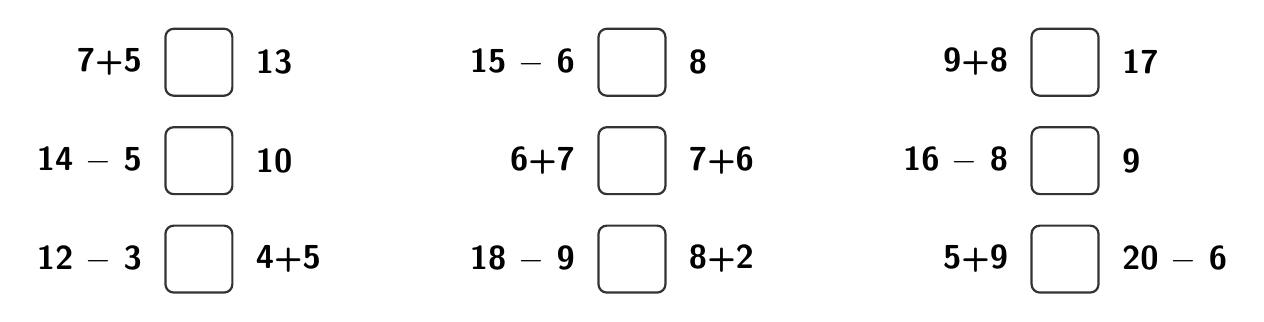
\begin{tikzpicture}[font=\sffamily\bfseries\large]
        \foreach \a/\b [count=\k] in {7+5/13,15 $-$ 6/8,9+8/17,14 $-$ 5/10,6+7/7+6,16 $-$ 8/9,12 $-$ 3/4+5,18 $-$ 9/8+2,5+9/20 $-$ 6}{
            \pgfmathtruncatemacro{\cot}{mod(\k-1,3)}\pgfmathtruncatemacro{\hang}{div(\k-1,3)}
            \begin{scope}[shift={(5.5*\cot,-1.25*\hang)}]
                \node[anchor=east] at (-0.6,0) {\a};
                \node[draw=black!80,thick,rounded corners=3pt,minimum size=0.85cm,inner sep=0pt] at (0,0) {};
                \node[anchor=west] at (0.6,0) {\b};
            \end{scope}}
    \end{tikzpicture}\par}
\end{bt}
\begin{bt}
    Điền dấu $+$ hoặc $-$ thích hợp vào ô trống.
    \par\nopagebreak\vspace{4pt}\nopagebreak{\centering
    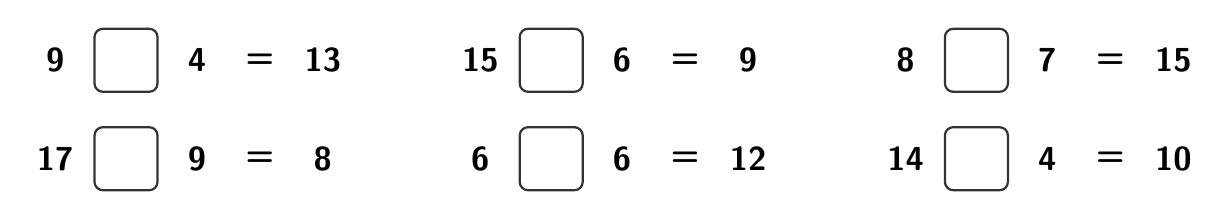
\begin{tikzpicture}[font=\sffamily\bfseries\large]
        \foreach \a/\b/\c [count=\k] in {9/4/13,15/6/9,8/7/15,17/9/8,6/6/12,14/4/10}{
            \pgfmathtruncatemacro{\cot}{mod(\k-1,3)}\pgfmathtruncatemacro{\hang}{div(\k-1,3)}
            \begin{scope}[shift={(5.4*\cot,-1.25*\hang)}]
                \node at (0,0) {\a};\node[draw=black!80,thick,rounded corners=3pt,minimum size=0.8cm,inner sep=0pt] at (0.9,0) {};
                \node at (1.8,0) {\b};\node at (2.6,0) {=};\node at (3.4,0) {\c};
            \end{scope}}
    \end{tikzpicture}\par}
\end{bt}
\OTdang{DẠNG 4. VẬN DỤNG VÀ MỞ RỘNG}
\begin{bt}
    Hoàn thành sơ đồ phép tính sau.
    \par\nopagebreak\vspace{4pt}\nopagebreak{\centering
        \OTchuoi{5}{$+\,4$}{$-\,3$}\\[10pt]
        \OTchuoi{12}{$+\,5$}{$-\,7$}\\[10pt]
        \OTchuoi{9}{$+\,6$}{$-\,8$}\\[10pt]
        \OTchuoi{18}{$-\,8$}{$+\,7$}\par}
\end{bt}
\begin{bt}
    Tháp số: số ở mỗi viên gạch bằng tổng hai số ở hai viên gạch ngay bên dưới. Điền số còn thiếu vào ô trống.
    \par\nopagebreak\vspace{4pt}\nopagebreak{\centering
    \begin{tikzpicture}
        \begin{scope}
            \node[OTgach] at (0,0) {3};\node[OTgach] at (1.6,0) {4};\node[OTgach] at (3.2,0) {5};
            \node[OTgach] at (0.8,0.85) {};\node[OTgach] at (2.4,0.85) {};
            \node[OTgach] at (1.6,1.7) {};
            \node[font=\sffamily\bfseries] at (1.6,-0.7) {a)};
        \end{scope}
        \begin{scope}[shift={(7,0)}]
            \node[OTgach] at (0,0) {2};\node[OTgach] at (1.6,0) {};\node[OTgach] at (3.2,0) {4};
            \node[OTgach] at (0.8,0.85) {8};\node[OTgach] at (2.4,0.85) {};
            \node[OTgach] at (1.6,1.7) {18};
            \node[font=\sffamily\bfseries] at (1.6,-0.7) {b)};
        \end{scope}
    \end{tikzpicture}\par}
\end{bt}
\begin{bt}
    Điền số vào các cửa sổ để tổng hai số bằng số ở mái nhà.
    \par\nopagebreak\vspace{4pt}\nopagebreak{\centering
        \OTnhaso{12}{5}{}\hfill\OTnhaso{15}{9}{}\hfill\OTnhaso{11}{}{4}\hfill\OTnhaso{14}{}{6}\\[8pt]
        \OTnhaso{13}{7}{}\hfill\OTnhaso{16}{}{9}\hfill\OTnhaso{18}{}{}\hfill\OTnhaso{20}{}{}\par}
\end{bt}
\begin{bt}
    Tô màu vào những ô có kết quả bằng $12$.
    \par\nopagebreak\vspace{4pt}\nopagebreak{\centering
    \begin{tikzpicture}
        \foreach \e [count=\k] in {7+5,8+5,15 $-$ 3,16 $-$ 7,6+6,11+2,9+3,13 $-$ 4,14 $-$ 2,9+4,17 $-$ 6,10+3}{
            \pgfmathtruncatemacro{\cot}{mod(\k-1,4)}\pgfmathtruncatemacro{\hang}{div(\k-1,4)}
            \begin{scope}[shift={(3.2*\cot,-1.6*\hang)}]\OTthepc{\e}\end{scope}}
    \end{tikzpicture}\par}
\end{bt}
\begin{bt}
    Quan sát tranh rồi viết phép tính thích hợp.
    \par\nopagebreak\vspace{6pt}\nopagebreak{\centering
    
\begin{tikzpicture}[font=\sffamily\bfseries\large]
        \draw[rounded corners=8pt,thick,gray!70,fill=black!3] (-0.5,0.8) rectangle (12.4,-1.0);
        \begin{scope}[shift={(-0.2,0)}]\OThang{\OTtao}{9}{0}\end{scope}
        \node at (6.2,0) {$+$};
        \begin{scope}[shift={(6.3,0)}]\OThang{\OTtao}{5}{0}\end{scope}
        \node[anchor=west] at (-0.3,-1.9) {Phép tính: \rule{1.2cm}{0.5pt} $+$ \rule{1.2cm}{0.5pt} $=$ \rule{1.2cm}{0.5pt}};
    \end{tikzpicture}\\[12pt]
    \begin{tikzpicture}[font=\sffamily\bfseries\large]
        \draw[rounded corners=8pt,thick,gray!70,fill=black!3] (-0.5,0.8) rectangle (12.4,-1.0);
        \begin{scope}[shift={(-0.2,0)}]\OThang{\OTbongbay}{14}{6}\end{scope}
        \node[anchor=west,font=\sffamily\small] at (1.0,-0.75) {(các quả bóng bị gạch chéo là đã bay mất)};
        \node[anchor=west] at (-0.3,-1.9) {Phép tính: \rule{1.2cm}{0.5pt} $-$ \rule{1.2cm}{0.5pt} $=$ \rule{1.2cm}{0.5pt}};
    \end{tikzpicture}\par}
\end{bt}
%%%%%%%%%%%%%%%%%%%%%%%%%%%%%
% BUỔI 2
%%%%%%%%%%%%%%%%%%%%%%%
\newpage
\TTdatlaibai
{\centering
        {\color{mauchinh!120}\bfseries\Large PHIẾU BÀI TẬP TOÁN TƯ DUY CẤP ĐỘ A}\\[3pt]
        {\color{mauchinh!120}\bfseries\Large CHỦ ĐỀ: ÔN TẬP CUỐI HỌC KÌ 1\\[2pt] PHẠM VI 100 (BUỔI 2)}\par}
\vspace{6pt}
\TTthongtin

\OTdang{DẠNG 1. ĐỌC, VIẾT, SO SÁNH, SẮP XẾP CÁC SỐ}
\begin{bt}
    Điền số còn thiếu vào ô trống.
    \par\nopagebreak\vspace{4pt}\nopagebreak{\centering
        \OTday{45,46,,48,,50,}\\[6pt]
        \OTday{20,18,,,12,,}\\[6pt]
        \OTday{10,20,,40,,60,}\\[6pt]
        \OTday{5,10,,20,,30,}\\[6pt]
        \OTday{99,98,,,95,,}\par}
\end{bt}
\begin{bt}
    Viết số liền trước, số ở giữa, số liền sau vào ô trống.
    \par\nopagebreak\vspace{4pt}\nopagebreak{\centering
        \OTlt{Số liền trước}{1}{{6},{45},{20},{57},{99}}\hfill
        \OTlt{Số ở giữa}{2}{{78/80},{2/4},{34/36},{67/69},{90/92}}\hfill
        \OTlt{Số liền sau}{3}{{58},{89},{45},{77},{19}}\par}
\end{bt}
\begin{bt}
    Điền dấu $>$, $<$, $=$ thích hợp vào ô trống.
    \par\nopagebreak\vspace{4pt}\nopagebreak{\centering
    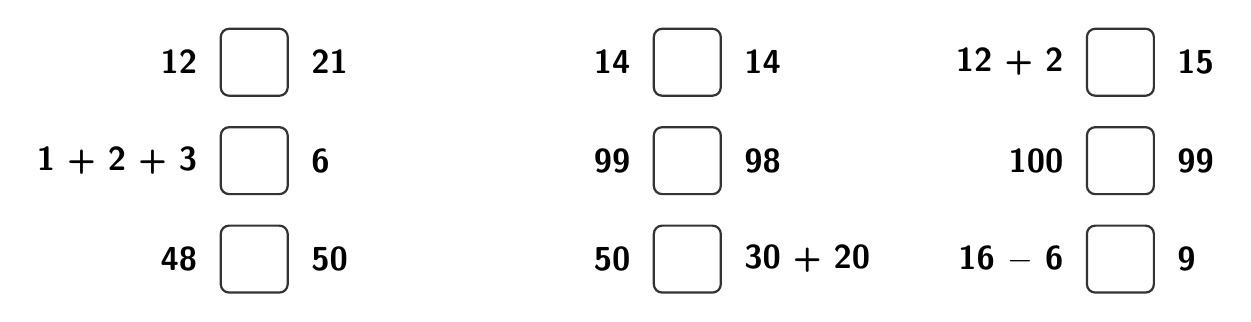
\begin{tikzpicture}[font=\sffamily\bfseries\large]
        \foreach \a/\b [count=\k] in {12/21,14/14,12 + 2/15,1 + 2 + 3/6,99/98,100/99,48/50,50/30 + 20,16 $-$ 6/9}{
            \pgfmathtruncatemacro{\cot}{mod(\k-1,3)}\pgfmathtruncatemacro{\hang}{div(\k-1,3)}
            \begin{scope}[shift={(5.5*\cot,-1.25*\hang)}]
                \node[anchor=east] at (-0.6,0) {\a};
                \node[draw=black!80,thick,rounded corners=3pt,minimum size=0.85cm,inner sep=0pt] at (0,0) {};
                \node[anchor=west] at (0.6,0) {\b};
            \end{scope}}
    \end{tikzpicture}\par}
\end{bt}
\begin{bt}
    Tô màu \textbf{hồng} vào hoa ghi số chẵn, tô màu \textbf{xanh} vào hoa ghi số lẻ.
    \par\nopagebreak\vspace{4pt}\nopagebreak{\centering\begin{minipage}{\linewidth}\centering
        \OThoa{75}{white}\hfill\OThoa{26}{white}\hfill\OThoa{32}{white}\hfill\OThoa{39}{white}\hfill\OThoa{50}{white}\\[4pt]
        \OThoa{41}{white}\hfill\OThoa{18}{white}\hfill\OThoa{65}{white}\hfill\OThoa{88}{white}\hfill\OThoa{9}{white}\\[4pt]
        \OThoa{16}{white}\hfill\OThoa{11}{white}\hfill\OThoa{22}{white}\hfill\OThoa{93}{white}\hfill\OThoa{70}{white}\end{minipage}\par}
\end{bt}
\begin{bt}
    Sắp xếp các số theo thứ tự \textbf{từ bé đến lớn}.
    \par\nopagebreak\vspace{4pt}\nopagebreak{\centering
    \begin{tikzpicture}[font=\sffamily\bfseries\Large]
        \foreach \a/\b/\c/\d [count=\k] in {27/72/17/70,45/54/40/5,88/8/80/18}{
            \node[OTthe] at (0,-1.7*\k) {\a};\node[OTthe] at (1.6,-1.7*\k) {\b};
            \node[OTthe] at (3.2,-1.7*\k) {\c};\node[OTthe] at (4.8,-1.7*\k) {\d};
            \draw[-latex,very thick,black!70] (5.8,-1.7*\k)--(6.6,-1.7*\k);
            \foreach \x in {0,1,2,3}{\node[OTo,minimum width=1.2cm,minimum height=0.95cm] at ({7.4+1.7*\x},-1.7*\k) {};}
            \foreach \x in {0,1,2}{\node at ({8.25+1.7*\x},-1.7*\k) {$<$};}}
    \end{tikzpicture}\par}
\end{bt}
\begin{bt}
    Viết số thích hợp vào chỗ chấm.
    \begin{listEX}
        \item Số gồm 7 chục và 4 đơn vị là: \TTcham[2cm]
        \item Số tròn chục liền sau số 40 là: \TTcham[2cm]
        \item Số lớn nhất có một chữ số là: \TTcham[2cm]
        \item Số bé nhất có hai chữ số là: \TTcham[2cm]
    \end{listEX}
\end{bt}
\OTdang{DẠNG 2. CỘNG, TRỪ TRONG PHẠM VI 100}
\begin{bt}
    Tính nhẩm.
    \par\nopagebreak\vspace{4pt}\nopagebreak{\centering
        \OTcotpt{30+50,20+70,60+30,40+40,10+80}\hfill
        \OTcotpt{90-40,80-30,70-50,60-20,100-10}\hfill
        \OTcotpt{50+50,100-60,30+20+10,90-30-20,40+10+30}\par}
\end{bt}
\begin{bt}
    Điền số thích hợp vào ô trống.
    \begin{listEX}
        \item $43+5=40+3+5=40+\OTovuong=\OTovuong$
        \item $62+7=60+2+7=60+\OTovuong=\OTovuong$
        \item $85-4=80+5-4=80+\OTovuong=\OTovuong$
        \item $79-6=70+9-6=70+\OTovuong=\OTovuong$
        \item $34+20=30+20+4=\OTovuong+4=\OTovuong$
        \item $68-30=60-30+8=\OTovuong+8=\OTovuong$
    \end{listEX}
\end{bt}
\begin{bt}
    Tính nhẩm (cộng số có hai chữ số).
    \par\nopagebreak\vspace{4pt}\nopagebreak{\centering
        \OTcotpt{24+30,56+20,41+50,63+30,18+80}\hfill
        \OTcotpt{70+25,40+37,20+68,50+49,30+12}\hfill
        \OTcotpt{32+7,45+4,68+1,71+8,50+9}\par}
\end{bt}
\begin{bt}
    Tính nhẩm (trừ số có hai chữ số).
    \par\nopagebreak\vspace{4pt}\nopagebreak{\centering
        \OTcotpt{48-5,67-7,95-40,79-30,100-20}\hfill
        \OTcotpt{86-6,59-9,74-4,68-8,97-7}\hfill
        \OTcotpt{85-50,99-60,76-30,57-20,64-10}\par}
\end{bt}
\begin{bt}
    Viết phép tính theo các bước nhảy trên tia số rồi tính.
    \par\nopagebreak\vspace{6pt}\nopagebreak{\centering
    
\begin{tikzpicture}[font=\sffamily\bfseries]
        \OTtia{100}{10}{0.115}
        \OTcung{30}{50}{0.115}{+20}{bend left}\OTcung{50}{70}{0.115}{+20}{bend left}
        \node[anchor=west,font=\sffamily\bfseries\large] at (-0.3,-1.25) {30 + 40 = \rule{1.2cm}{0.5pt}};
    \end{tikzpicture}\\[12pt]
    
\begin{tikzpicture}[font=\sffamily\bfseries]
        \OTtia{100}{10}{0.115}
        \OTcung{90}{70}{0.115}{$-20$}{bend right}\OTcung{70}{40}{0.115}{$-30$}{bend right}
        \node[anchor=west,font=\sffamily\bfseries\large] at (-0.3,-1.25) {90 $-$ 50 = \rule{1.2cm}{0.5pt}};
    \end{tikzpicture}\\[12pt]
    \begin{tikzpicture}[font=\sffamily\bfseries]
        \OTtia{100}{10}{0.115}
        \node[anchor=west,font=\sffamily\bfseries\large] at (-0.3,-1.25) {Tự nhảy: 20 + 60 = \rule{1.2cm}{0.5pt} \qquad 80 $-$ 50 = \rule{1.2cm}{0.5pt}};
    \end{tikzpicture}\par}
\end{bt}
\begin{bt}
    Điền số thích hợp vào bảng.
    \par\nopagebreak\vspace{4pt}\nopagebreak{\centering
    \renewcommand{\arraystretch}{1.7}
    \begin{tabular}{|*{4}{>{\centering\arraybackslash}p{2.6cm}|}}
        \hline
        \textbf{Số đã cho} & \textbf{Cộng thêm 10} & \textbf{Cộng thêm 20} & \textbf{Bớt đi 10} \\ \hline
        15 & & & \\ \hline
        34 & & & \\ \hline
        52 & & & \\ \hline
        67 & & & \\ \hline
        70 & & & \\ \hline
    \end{tabular}\par}
\end{bt}
\OTdang{DẠNG 3. TÌM SỐ CÒN THIẾU, SO SÁNH PHÉP TÍNH}
\begin{bt}
    Tìm số còn thiếu (điền vào ô trống).
    \par\nopagebreak\vspace{6pt}\nopagebreak{\centering
    \renewcommand{\arraystretch}{2.0}
    \begin{tabular}{*{3}{>{\centering\arraybackslash}p{0.3\linewidth}}}
        $\OTovuong[0.7cm]+30=80$ & $70-\OTovuong[0.7cm]=40$ & $25+\OTovuong[0.7cm]=29$ \\
        $58-\OTovuong[0.7cm]=53$ & $40+\OTovuong[0.7cm]=90$ & $\OTovuong[0.7cm]-20=50$ \\
        $\OTovuong[0.7cm]+6=36$ & $90-\OTovuong[0.7cm]=60$ & $\OTovuong[0.7cm]-4=45$ \\
    \end{tabular}\par}
\end{bt}
\begin{bt}
    Điền dấu $>$, $<$, $=$ thích hợp vào ô trống.
    \par\nopagebreak\vspace{4pt}\nopagebreak{\centering
    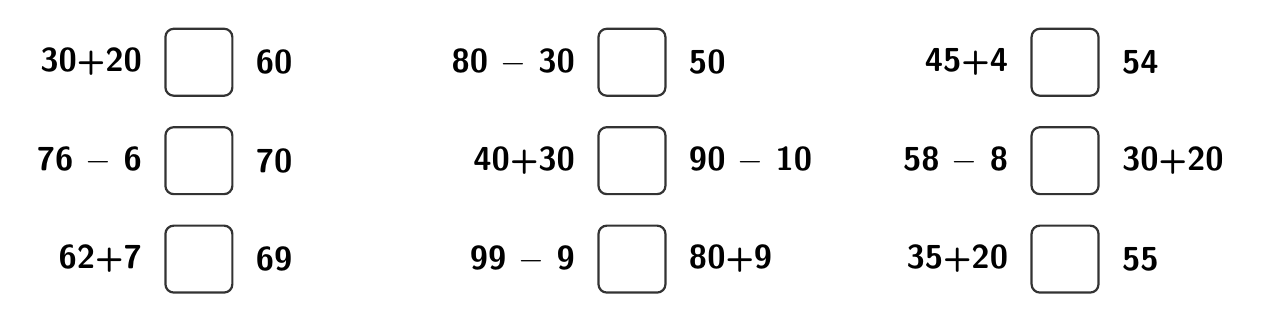
\begin{tikzpicture}[font=\sffamily\bfseries\large]
        \foreach \a/\b [count=\k] in {30+20/60,80 $-$ 30/50,45+4/54,76 $-$ 6/70,40+30/90 $-$ 10,58 $-$ 8/30+20,62+7/69,99 $-$ 9/80+9,35+20/55}{
            \pgfmathtruncatemacro{\cot}{mod(\k-1,3)}\pgfmathtruncatemacro{\hang}{div(\k-1,3)}
            \begin{scope}[shift={(5.5*\cot,-1.25*\hang)}]
                \node[anchor=east] at (-0.6,0) {\a};
                \node[draw=black!80,thick,rounded corners=3pt,minimum size=0.85cm,inner sep=0pt] at (0,0) {};
                \node[anchor=west] at (0.6,0) {\b};
            \end{scope}}
    \end{tikzpicture}\par}
\end{bt}
\OTdang{DẠNG 4. VẬN DỤNG VÀ MỞ RỘNG}
\begin{bt}
    Hoàn thành sơ đồ phép tính sau.
    \par\nopagebreak\vspace{4pt}\nopagebreak{\centering
        \OTchuoi{25}{$+\,30$}{$-\,20$}\\[10pt]
        \OTchuoi{40}{$+\,50$}{$-\,30$}\\[10pt]
        \OTchuoi{63}{$+\,6$}{$-\,3$}\\[10pt]
        \OTchuoi{90}{$-\,40$}{$+\,7$}\par}
\end{bt}
\begin{bt}
    Tháp số: số ở mỗi viên gạch bằng tổng hai số ở hai viên gạch ngay bên dưới. Điền số còn thiếu vào ô trống.
    \par\nopagebreak\vspace{4pt}\nopagebreak{\centering
    \begin{tikzpicture}
        \begin{scope}
            \node[OTgach] at (0,0) {10};\node[OTgach] at (1.6,0) {20};\node[OTgach] at (3.2,0) {30};
            \node[OTgach] at (0.8,0.85) {};\node[OTgach] at (2.4,0.85) {};
            \node[OTgach] at (1.6,1.7) {};
            \node[font=\sffamily\bfseries] at (1.6,-0.7) {a)};
        \end{scope}
        \begin{scope}[shift={(7,0)}]
            \node[OTgach] at (0,0) {10};\node[OTgach] at (1.6,0) {};\node[OTgach] at (3.2,0) {20};
            \node[OTgach] at (0.8,0.85) {40};\node[OTgach] at (2.4,0.85) {};
            \node[OTgach] at (1.6,1.7) {90};
            \node[font=\sffamily\bfseries] at (1.6,-0.7) {b)};
        \end{scope}
    \end{tikzpicture}\par}
\end{bt}
%%%%%%%%%%%%%%%%%%%%%%%%%%%%%
% BUỔI 3
%%%%%%%%%%%%%%%%%%%%%%%
\newpage
\TTdatlaibai
{\centering
        {\color{mauchinh!120}\bfseries\Large PHIẾU BÀI TẬP TOÁN TƯ DUY CẤP ĐỘ A}\\[3pt]
        {\color{mauchinh!120}\bfseries\Large CHỦ ĐỀ: ÔN TẬP CUỐI HỌC KÌ 1\\[2pt] THỜI GIAN, HÌNH HỌC VÀ TỔNG HỢP (BUỔI 3)}\par}
\vspace{6pt}
\TTthongtin

\OTdang{DẠNG 1. XEM ĐỒNG HỒ}
\begin{bt}
    Đồng hồ chỉ mấy giờ?
    \par\nopagebreak\vspace{4pt}\nopagebreak{\centering
    \begin{tabular}{*{3}{>{\centering\arraybackslash}p{0.31\linewidth}}}
        \OTdh{3}{0} & \OTdh{7}{0} & \OTdh{11}{0}\\[2pt]
        \TTcham[1.2cm] giờ & \TTcham[1.2cm] giờ & \TTcham[1.2cm] giờ\\[10pt]
        \OTdh{6}{30} & \OTdh{9}{30} & \OTdh{12}{30}\\[2pt]
        \TTcham[1.2cm] giờ 30 phút & \TTcham[1.2cm] giờ 30 phút & \TTcham[1.2cm] giờ 30 phút\\
    \end{tabular}\par}
\end{bt}
\begin{bt}
    Nối đồng hồ với giờ tương ứng.
    \par\nopagebreak\vspace{4pt}\nopagebreak{\centering
    \begin{tikzpicture}[font=\sffamily\bfseries\large]
        \foreach \h/\m/\y in {2/0/0,8/30/-2.5,5/0/-5.0}{
            \node at (0,\y) {\OTdh{\h}{\m}};\fill (1.35,\y) circle (2.5pt);}
        \foreach \t/\y in {{5 giờ}/-0.4,{2 giờ}/-2.1,{8 giờ 30 phút}/-4.9}{
            \fill (6.6,\y) circle (2.5pt);
            \node[draw=black!80,thick,rounded corners=5pt,fill=OTvangnhat,minimum width=3.8cm,minimum height=0.8cm,anchor=west] at (7.0,\y) {\t};}
    \end{tikzpicture}\par}
\end{bt}
\begin{bt}
    Vẽ kim giờ và kim phút ứng với thời gian ghi dưới mỗi đồng hồ.
    \par\nopagebreak\vspace{4pt}\nopagebreak{\centering
    \begin{tabular}{*{3}{>{\centering\arraybackslash}p{0.31\linewidth}}}
        \OTdh[0]{1}{0} & \OTdh[0]{4}{0} & \OTdh[0]{10}{0}\\[2pt]
        1 giờ & 4 giờ & 10 giờ\\[10pt]
        \OTdh[0]{2}{30} & \OTdh[0]{7}{30} & \OTdh[0]{11}{30}\\[2pt]
        2 giờ 30 phút & 7 giờ 30 phút & 11 giờ 30 phút\\
    \end{tabular}\par}
\end{bt}
\begin{bt}
    Khoanh tròn vào đồng hồ chỉ đúng thời gian.
    \par\nopagebreak
    \begin{listEX}
        \item Lúc $8$ giờ:\par\nopagebreak\smallskip
            {\centering\OTdh{8}{0}\hspace{1.2cm}\OTdh{4}{0}\hspace{1.2cm}\OTdh{8}{30}\par}
        \item Lúc $3$ giờ $30$ phút:\par\nopagebreak\smallskip
            {\centering\OTdh{3}{0}\hspace{1.2cm}\OTdh{6}{15}\hspace{1.2cm}\OTdh{3}{30}\par}
    \end{listEX}
\end{bt}
\OTdang{DẠNG 2. HÌNH HỌC}
\begin{bt}
    Đếm số hình rồi điền vào bảng.
    \par\nopagebreak\vspace{4pt}\nopagebreak{\centering
    
\begin{tikzpicture}
        \draw[rounded corners=8pt,thick,gray!70,fill=black!3] (-0.8,0.9) rectangle (12.8,-3.5);
        \foreach \t/\x/\y in {C/0.3/0,T/2.2/0.1,V/4.2/-0.05,N/6.3/0.05,C/8.4/0,T/10.2/0.1,C/12.0/-0.05,
                              V/0.4/-2.4,T/2.3/-2.5,C/4.2/-2.4,N/6.3/-2.55,V/8.3/-2.4,C/10.2/-2.5,T/12.0/-2.4}{
            \begin{scope}[shift={(\x,\y-0.4)}]\OThinh{\t}\end{scope}}
    \end{tikzpicture}\par\bigskip
    \renewcommand{\arraystretch}{1.5}
    \begin{tabular}{|>{\centering\arraybackslash}p{3cm}|>{\centering\arraybackslash}p{2.6cm}|>{\centering\arraybackslash}p{2.6cm}|>{\centering\arraybackslash}p{2.6cm}|>{\centering\arraybackslash}p{2.6cm}|}
        \hline
        \textbf{Hình} &
        \begin{tikzpicture}[baseline=-0.1cm]\OThinh{T}\end{tikzpicture} &
        \begin{tikzpicture}[baseline=-0.1cm]\OThinh{V}\end{tikzpicture} &
        \begin{tikzpicture}[baseline=-0.1cm]\OThinh{N}\end{tikzpicture} &
        \begin{tikzpicture}[baseline=-0.1cm]\OThinh{C}\end{tikzpicture}\\ \hline
        \textbf{Số lượng} & & & & \\ \hline
    \end{tabular}\par}
\end{bt}
\OTdang{DẠNG 3. TỔNG HỢP}
\begin{bt}
    Khoanh tròn vào chữ cái đặt trước đáp án đúng.
    \par\nopagebreak
    \begin{listEX}
        \item Số liền sau của $79$ là:\OTchon{$78$}{$80$}{$70$}
        \item Số nào dưới đây là số chẵn?\OTchon{$15$}{$21$}{$18$}
        \item Kết quả của phép tính $15-6$ là:\OTchon{$8$}{$9$}{$10$}
        \item Số $56$ gồm:\OTchon{$5$ chục và $6$ đơn vị}{$6$ chục và $5$ đơn vị}{$50$ đơn vị}
        \item Đồng hồ chỉ $7$ giờ thì kim ngắn chỉ số $7$, kim dài chỉ số:\OTchon{$12$}{$6$}{$7$}
    \end{listEX}
\end{bt}
\begin{bt}
    Đúng ghi Đ, sai ghi S vào ô trống.
    \par\nopagebreak\vspace{4pt}\nopagebreak{\centering
    \renewcommand{\arraystretch}{1.75}
    \begin{tabular}{|>{\raggedright\arraybackslash}p{8.8cm}|>{\centering\arraybackslash}p{2.6cm}|}
        \hline
        $9 + 6 = 15$ & \OTovuong \\ \hline
        $12 - 5 = 8$ & \OTovuong \\ \hline
        $45 > 54$ & \OTovuong \\ \hline
        $50 = 30 + 20$ & \OTovuong \\ \hline
        Số $38$ là số chẵn & \OTovuong \\ \hline
        Số tròn chục bé nhất là $10$ & \OTovuong \\ \hline
    \end{tabular}\par}
\end{bt}
\begin{bt}
    Giải các bài toán sau.
    \begin{listEX}
        \item Hà có 8 quả bóng bay, mẹ mua thêm cho Hà 7 quả bóng bay. Hỏi Hà có tất cả bao nhiêu quả bóng bay?
        \OTkhungpt
        \item Trong vườn có 15 con gà, có 6 con gà chạy ra ngoài cổng. Hỏi trong vườn còn lại bao nhiêu con gà?
        \OTkhungpt
        \item Lớp 1A có 30 bạn nam và 20 bạn nữ. Hỏi lớp 1A có tất cả bao nhiêu bạn?
        \OTkhungpt
    \end{listEX}
\end{bt}
\begin{center}
       \faGg\faGg\quad Hết \quad\faGg\faGg
\end{center}
\end{document}
